\chapter{Superfícies}
  Neste capítulo, estudamos funções vetoriais do tipo $\vec{f}(u,v)$, ou seja, uma função que associa um ponto do plano real a vetores no espaço.
\section{Funções vetoriais de duas variáveis reais - superfícies}
Uma função vetorial de duas variáveis é uma função da forma $$\vec{r}:D_1\times D_2 \to \mathbb{R}^3,$$ onde $D_1\times D_2\subseteq \mathbb{R}^2$ é o domínio de definição de $\vec{r}$ e $(u,v)\in D_1\times D_2$ são os parâmetros ou as coordenadas de superfície. Em coordenadas cartesianas, uma função vetorial assume a seguinte forma:
$$\vec{r}(u,v)=x(u,v)\vec{i}+y(u,v)\vec{j}+z(u,v)\vec{k}$$
\begin{ex}\label{exfv_1} São exemplos de funções vetoriais
\begin{itemize}
\item [a)] $\vec{f}(u,v)=\sin(u)\vec{i}+\cos(v)\vec{j}+uv\vec{k}$
\item [b)] $\vec{g}(u,v)=\sin(u)\cos(v) \vec{i}+\cosh(u)\sinh(v)\vec{j}+u\vec{k}$
\end{itemize}
\end{ex}
Uma superfície\index{superfície} no espaço pode ser representada pelo conjunto de pontos de uma função vetorial $\vec{r}(u,v)$ não constante em todo o seu domínio. A seguinte interpretação ajuda entender essa função: se fixamos $v$ e temos que $\vec{r}(u,v)$ descreve uma curva e $\vec{r}_u(u,v)$ é um vetor tangente a essa curva. Da mesma forma, se fixamos $u$ temos que $\vec{r}(u,v)$ descreve uma curva e $\vec{r}_v(u,v)$ é um vetor tangente a essa curva. Se essas curvas não forem paralelas, temos um sistema de coordenadas curvilíneo para escrever todos os pontos da superfície. Pense no globo terrestre, o medidiano de Greenwich e a linha do Equador: o globo como uma superfície, Greenwich e Equador como duas curvas e longitude e latitude como um sistema de coordenadas curvilíneo, veja Figura~\ref{cap_superficies_esfera} Observe que esse sistema curvilíneo fica bem definido quando $\vec{r}_u$ e $\vec{r}_v$ não são paralelos nos pontos do domínio. Chamamos de superfície regular aquela que satisfaz
$$
\vec{r}_u\times \vec{r}_v\neq \vec{0}.
$$
\begin{ex}A superfície
$$
\vec{r}=a\sin(u)\cos(v)\vec{i}+a\sin(u)\sin(v)\vec{j}+a\cos(u)\vec{k},~~ a>0, ~ 0\leq u< \pi, ~ 0\leq v< 2\pi
$$
descreve uma esfera centrada na origem e raio $a$. De fato, colocando $$x=a\sin(u)\cos(v),\qquad y=a\sin(u)\sin(v)\qquad\text{e}\qquad z=a\cos(u),$$
temos que
$$
x^2+y^2+z^2=a^2.
$$
\end{ex}
Além disso, se $(x,y,z)$ é um ponto qualquer nesta esfera, então existem $u$ e $v$ na parametrização. Para tal, basta escolher $u=\cos^{-1}\left(\frac{z}{a}\right)$ e escolher $v\in[0,2\pi)$ tal que:
$$\cos(v)=\frac{x}{a\sin(u)} \quad \hbox{e} \quad \sin(v)=\frac{y}{a\sin(u)},~~u\neq 0 ~~ \hbox{e} ~~u\neq \pi.$$

 \begin{figure}%{r}{8cm}
\centering
 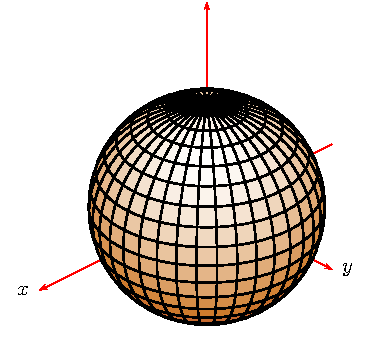
\includegraphics{cap_superficies/figs/figura_1}\label{cap_superficies_esfera}
\caption{Um esfera centrada na origem com meridianos e paralelos traçados.}
\end{figure}
% \begin{prob}Verifique que
% $$
% \vec{r}=\cosh(u)\cos( v)\vec{i}+ \cosh(u)\sin(v)\vec{j}+\sinh(u)\vec{k},\ 0\leq v\leq 2\pi,\ u\in\mathcal{R}
% $$
% descreve um hiperbolóide de uma folha.
% \end{prob}
\section{Quádricas}
A figura \ref{quadricas} apresenta uma lista das principais quádricas\index{quádricas} estudadas na disciplina de Cálculo Diferencial e Integral com funções de várias variáveis. As equações são as seguintes:
\begin{itemize}
\item[a)] Cone elíptico: $\displaystyle z^2=\frac{x^2}{a^2}+\frac{y^2}{b^2}$.
\item[b)] Elipsóide: $\displaystyle \frac{x^2}{a^2}+\frac{y^2}{b^2}+\frac{z^2}{c^2}=1$
\item[c)] Parabolóide Elíptico: $\displaystyle z=\frac{x^2}{a^2}+\frac{y^2}{b^2}$
\item[d)] Parabolóide Hiperbólico: $\displaystyle z=\frac{x^2}{a^2}-\frac{y^2}{b^2}$
\item[e)] Hiperbolóide de uma folha: $\displaystyle \frac{x^2}{a^2}+\frac{y^2}{b^2}-\frac{z^2}{c^2}=1$
\item[f)] Hiperbolóide de duas folhas:  $\displaystyle -\frac{x^2}{a^2}-\frac{y^2}{b^2}+\frac{z^2}{c^2}=1$
\end{itemize}
\begin{figure}[htp]
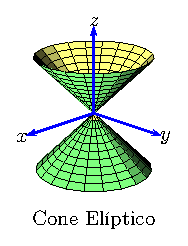
\includegraphics{cap_superficies/figs/figura_2}
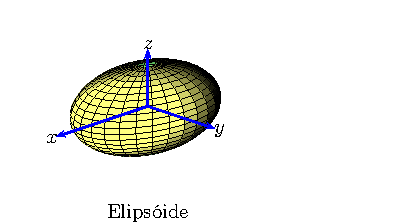
\includegraphics{cap_superficies/figs/figura_3}
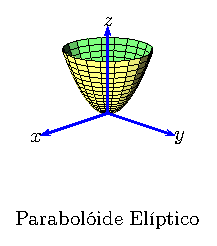
\includegraphics{cap_superficies/figs/figura_4}


\includegraphics{cap_superficies/figs/figura_5}
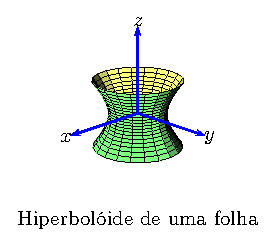
\includegraphics{cap_superficies/figs/figura_6}
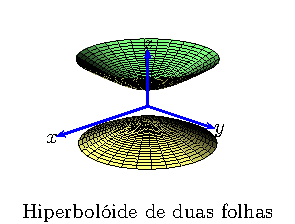
\includegraphics{cap_superficies/figs/figura_7} \caption{\label{quadricas}Quádricas}
\end{figure}
\section{Casos $y=f(x,z)$, $z=f(x,y)$ ou $x=f(y,z)$}
O caso particular da superfície representada por uma função $z=f(x,y)$, podemos assumir uma parametrização natural $\vec{r}=u\vec{i}+v\vec{j}+f(u,v)\vec{k}$. Analogamente para os casos $y=f(x,z)$ ou $x=f(y,z)$, podemos assumir, respectivamente, as parametrizações $\vec{r}=u\vec{i}+f(u,v)\vec{j}+v\vec{k}$ ou $\vec{r}=f(u,v)\vec{i}+v\vec{j}+u\vec{k}$. Para o caso $z=f(x,y)$ (analogamente para os demais), a condição $\vec{r}_u\times \vec{r}_v\neq \vec{0}$ assume a forma
\begin{eqnarray*}
 \vec{r}_u\times \vec{r}_v&=&\left|\begin{array}{ccc}\vec{i}&\vec{j}&\vec{k}\\ 1&0&f_u(u,v)\\0&1&f_v(u,v)\end{array} \right|\\&=&-f_u\vec{i}-f_v\vec{j}+\vec{k}\neq \vec{0}.
\end{eqnarray*}
Isso implica que $ \vec{r}_u\times \vec{r}_v \neq 0$, ou seja, a superfície \'{e} regular. Voltaremos a discutir esse assunto nos próximos capítulos, quando o vetor gradiente estiver definido.
\section{Vetor unitário normal}\index{vetor normal à uma superfície}
Para os fins de teoria de integraçao sobre superfícies, que discutiremos mais adiante, é fundamental definir o vetor unitário normal. Dado uma superfície e um ponto nela, dizemos que um vetor é normal à superfícies, se ele é perpendicular no ponto a cada curva contida na superfícies. Em especial, um vetor normal à superfícies no ponto $x_0=x(u_0,v_0)$, $y_0=y(u_0,v_0)$ e $z_0=z(u_0,v_0)$, deve ser perpendicular às curvas $\vec{r}(u_0,v)$ e $\vec{r}(u,v_0)$, isto é, as curvas geradas quando se fixa um dos parâmetros $u_0$ ou $v_0$, respectivamente. Assim, podemos concluir que cada vetor normal está da mesma direção do produto vetorial $\vec{r}_u\times\vec{r}_v$. Finalmente, o vetor normal unitário deve ter normal unitário, portanto, deve ser da forma:
\begin{equation}
 \vec{n} = \pm \frac{\vec{r}_u\times\vec{r}_v}{\|\vec{r}_u\times\vec{r}_v\|}.
\end{equation}
Aqui o sinal indica para qual lado o vetor normal aponta.
